\part{Literature Review}
In this part we will provide a description of the technologies used in this thesis. We will start describing what is ROS and how it works then we will talk about the navigation system used and how it is implemented the control with the fleet management system Open-RMF
\chapter{Overview of ROS1 and ROS2}
The Robotics Operating System \footnote{\href{https://www.ros.org/}{https://www.ros.org/}} is a compilation of tools and libraries open-source that help the development of application in the robotic environment. otherwise from the name, it's not a Operating System (OS) but an Software Development Kit (SDK) that gives at the user all the tools for creating your robot giving some typically functionality of an OS: hardware abstraction, low-level device control, implementation of commonly-used functionality, message-passing between processes, and package management.
The ROS ecosystem is based on (all these things is going to be described in detail in the next section):
\begin{itemize}
	\item An communication system named middleware or plumbing based on DDS (Data Distribution Service). This allow the Nodes to share information between each other with an anonymous publish/subscribe pattern allowing fault isolation, separation of concerns and clear interfaces and a synchronous system (remote procedure call)RPC-style communication between services.
	\item Tools to control and improve the development of the software like launch,  introspection, debugging, visualization, plotting, logging, and playback.
	\item Provides tools and libraries for obtaining, building, writing, and running code across multiple computers.
	\item A active and big community with at the center the Open Robotics\footnote{\href{https://www.openrobotics.org/}{https://www.openrobotics.org/}}.
\end{itemize}
\section{Structure of ROS}
The documentation\footnote{\href{https://docs.ros.org/en/rolling/index.html}{https://docs.ros.org/en/rolling/index.html}} give all the information of ROS, some functionality write below are not available for ROS 1:
\begin{itemize}
	\item The \textbf{ROS Graph} is a peer-to-peer network of processes that elaborated simultaneously and communicate with each other.
	\item \textbf{Nodes} is a modular process and should be a specific resolution for a problem to be more easily communicate with other Nodes through topics, services, action and parameters. They also can be based on LifecycleNode\label{LifecycleNode} that contain a state machine transitions for bringup and teardown to allow more deterministic behavior.
	\begin{figure}[h]
	\centering
	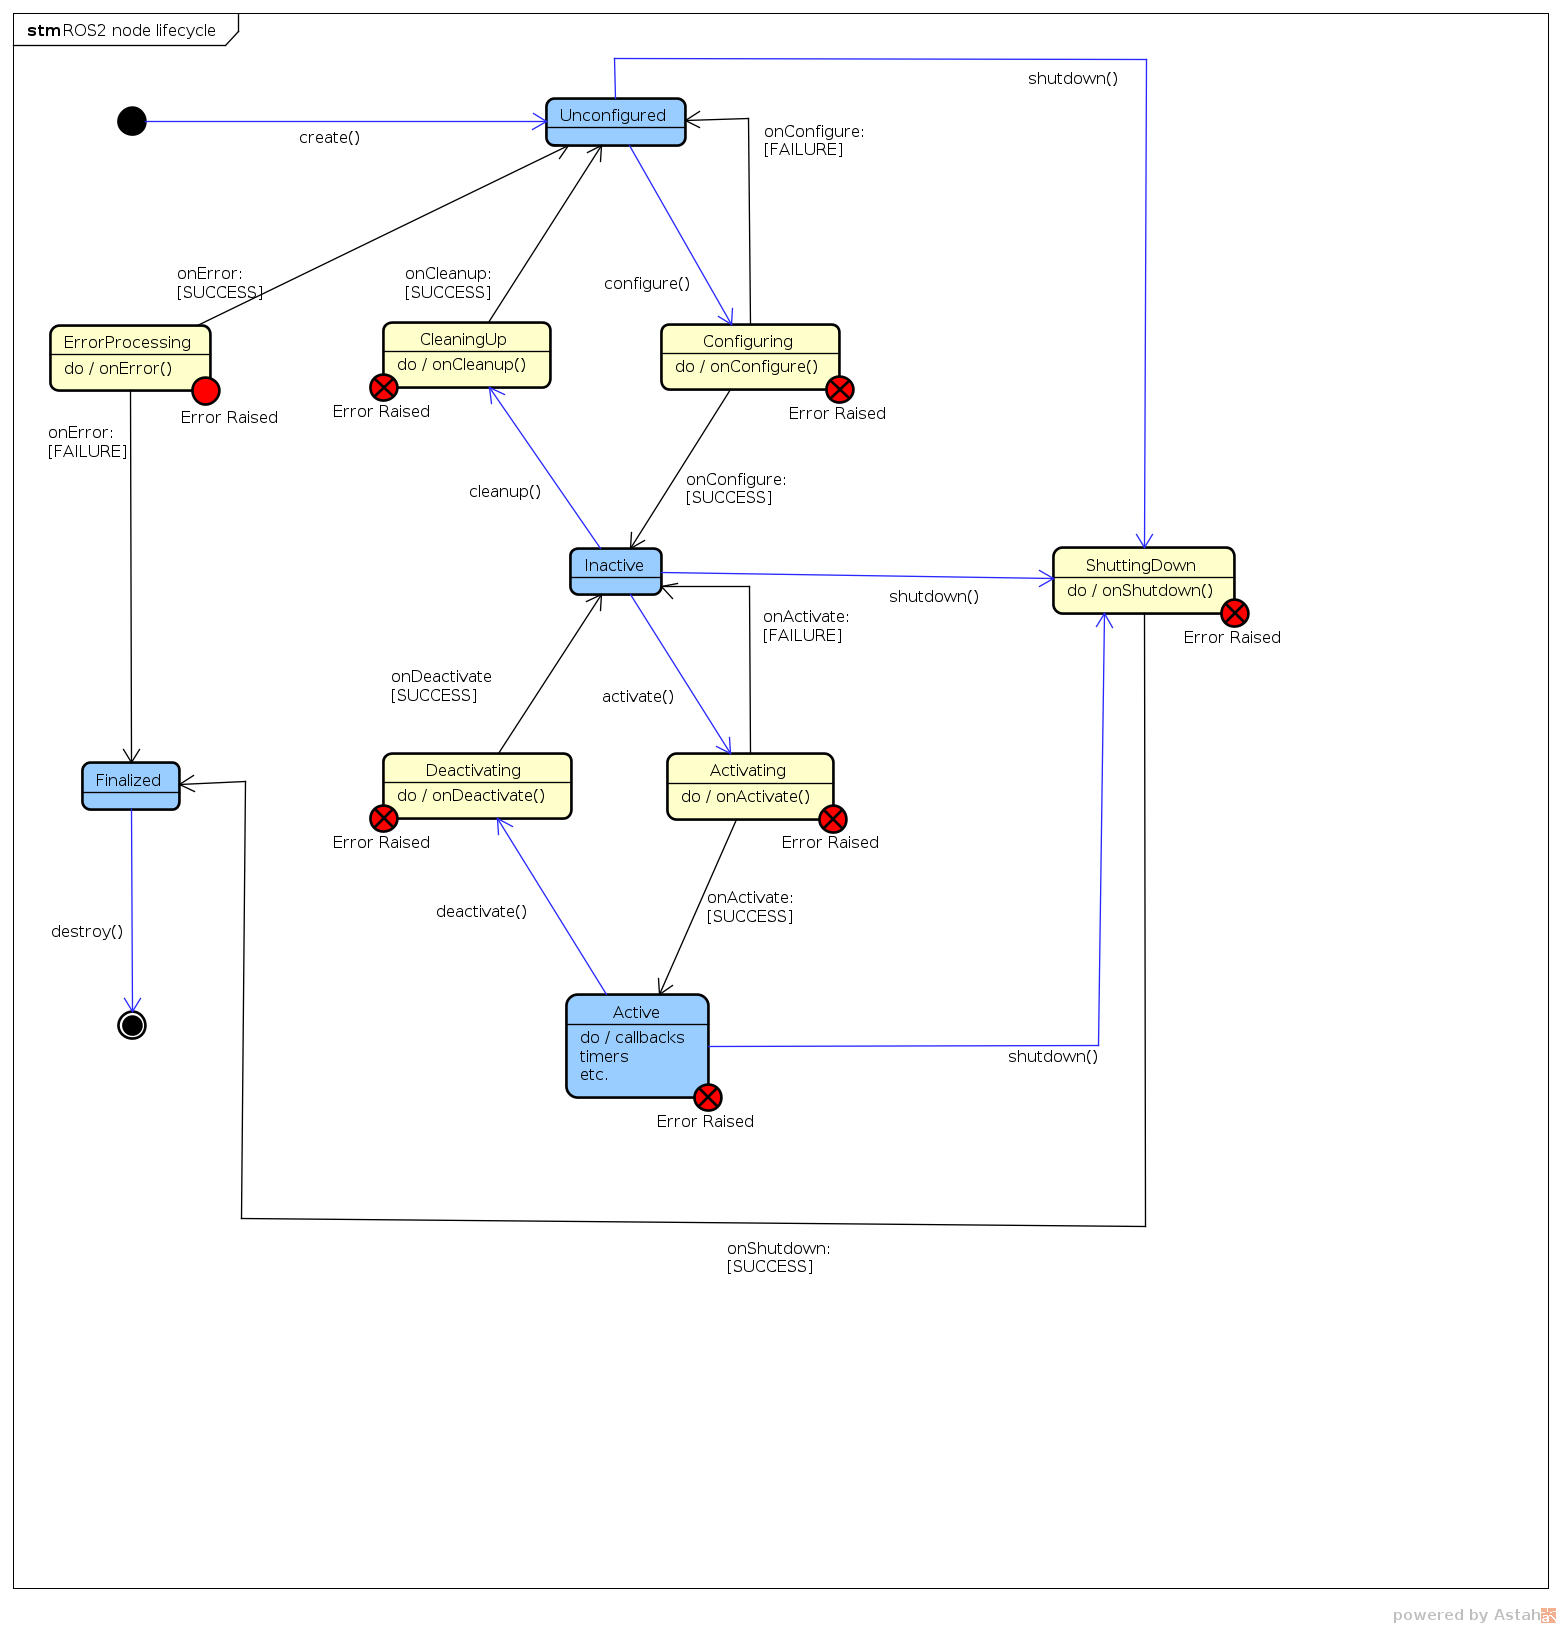
\includegraphics[width=0.8\linewidth]{img/life_cycle_sm.png}
	\captionof{figure}{State Machine of LifecycleNode}
	\end{figure}
	\item \textbf{Topics} are the bus for communication between Nodes to share a streams of messages in a publisher to subscriber structure.
	\begin{center}
		\captionsetup{type=figure}
		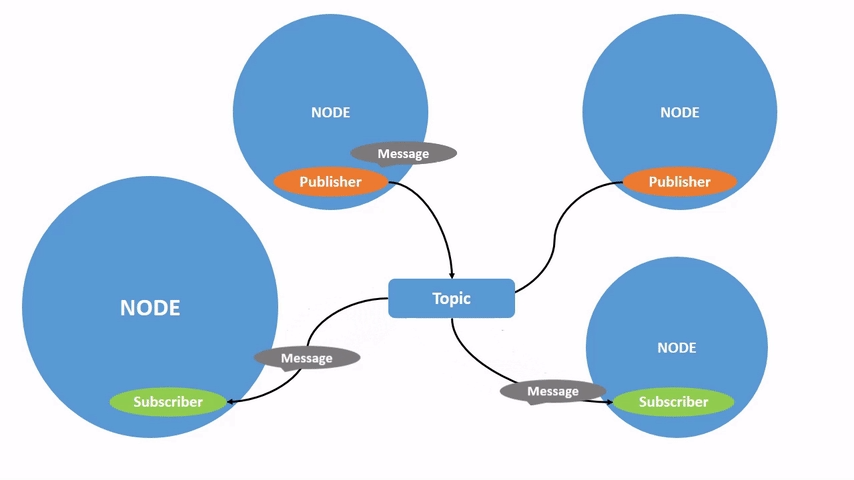
\includegraphics[width=0.49\linewidth]{img/Topic.png}
		\captionof{figure}{Topic process}
	\end{center}
	\item \textbf{Service} are based on the request and response model. When a node with a Service client send a Request Message to Node with a Service Server it will send a Response Message to that specific Service Client. 
	\begin{center}
		\captionsetup{type=figure}
		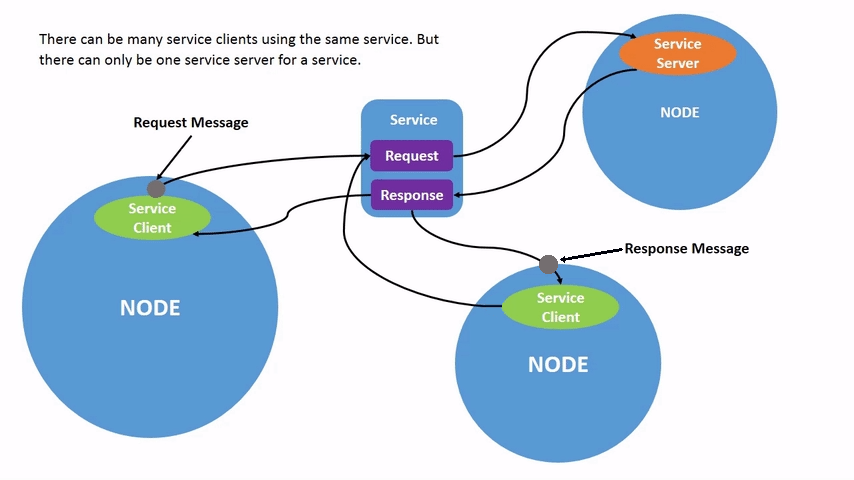
\includegraphics[width=0.49\linewidth]{img/Service.png}
		\captionof{figure}{Service process}
	\end{center}
	\item \textbf{Parameters} are configuration of a node and allow to modified them without changing the code.
	\item \textbf{Actions}\label{Action} were created to fulfill the needs of something for tracking long task. They are a combination of two service (goal and result) and a pub-sub (feedback). It send a goal request and receive a response then send a result request, the node then start to pub to the feedback topic and then response to the result request.
	\begin{center}
		\captionsetup{type=figure}
		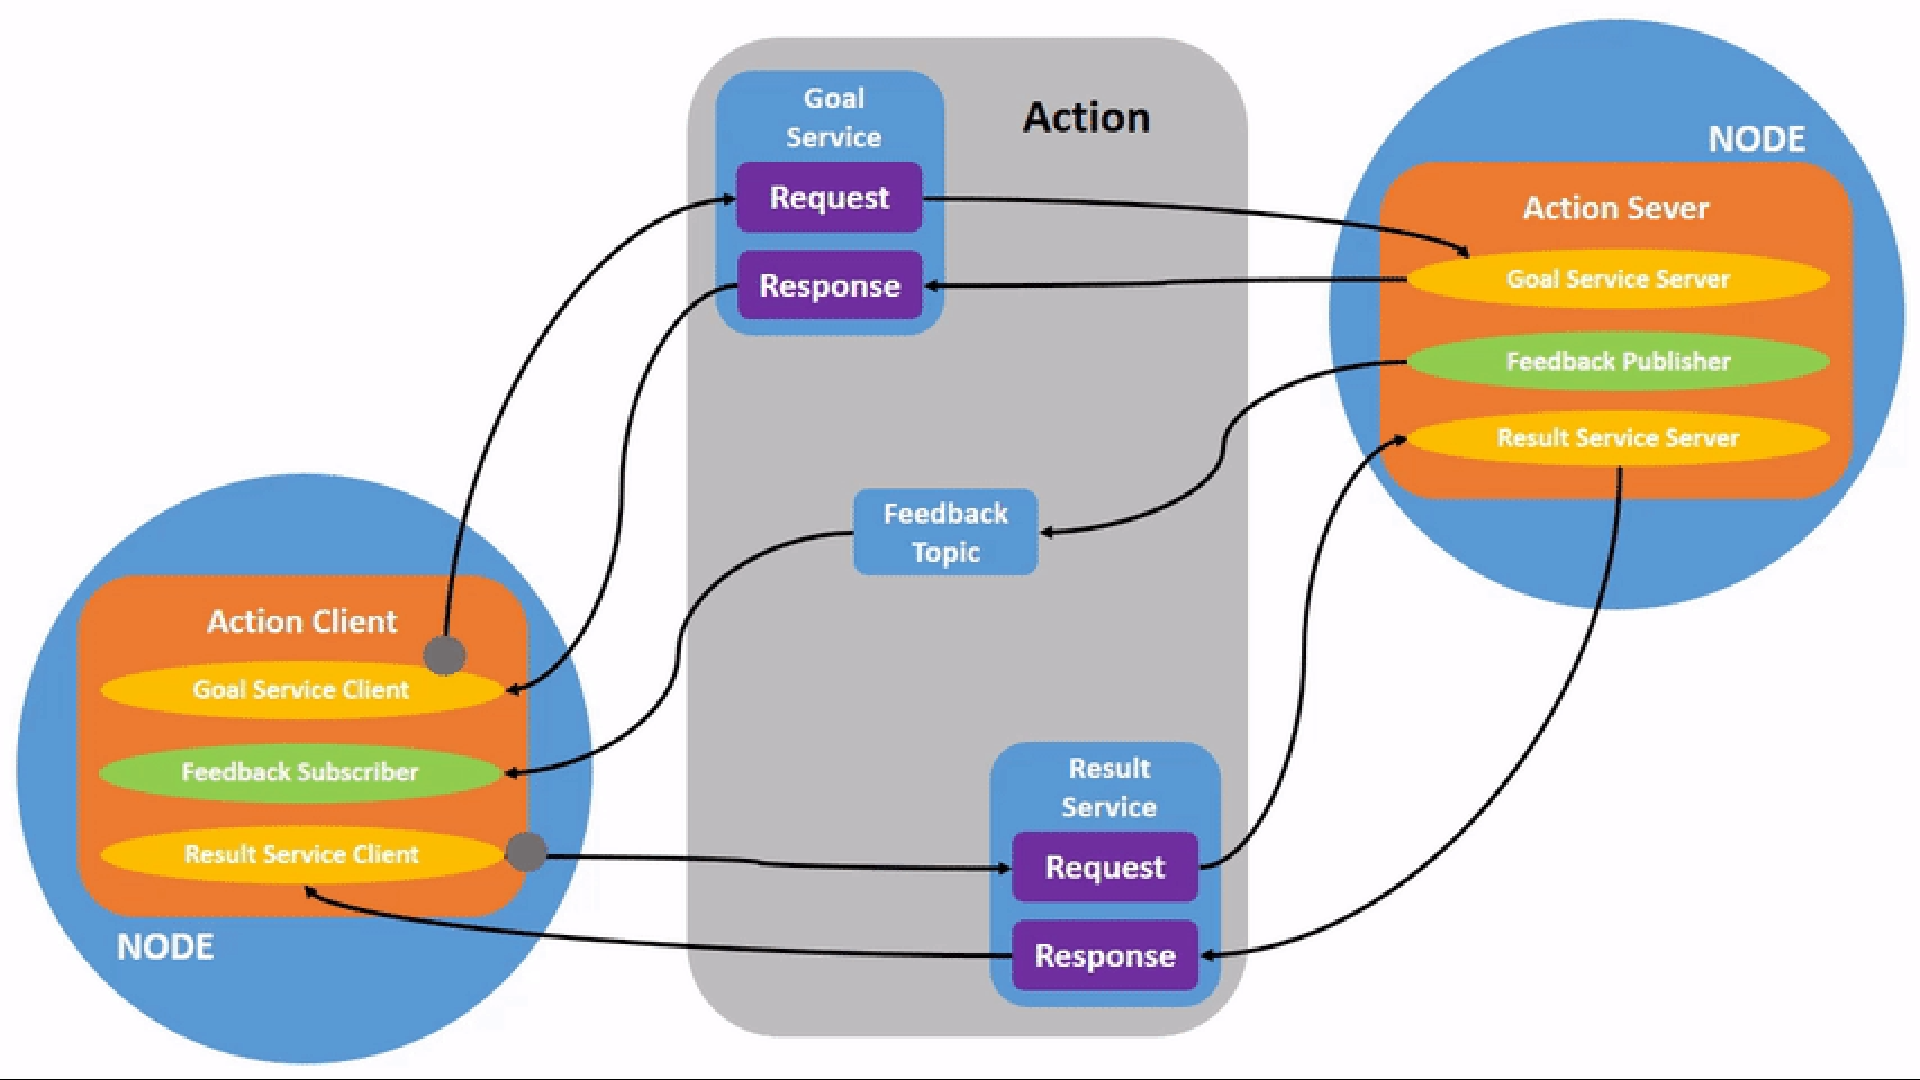
\includegraphics[width=0.49\linewidth]{img/Action.png}
		\captionof{figure}{Action process}
	\end{center}
\end{itemize}
\section{Tools of ROS}
Now i will describe the tools that are built in ROS for developing robotics system:
\begin{itemize}
	\item \textbf{Launch} is a file structure that allow to start multiple nodes with a set of parameters.
	\item \textbf{rqt} is a graphical user interface (GUI) tool for ROS 2. With a series of plugins allow to interact with an interface for helping in the development, in the monitoring and diagnostic the ROS system.
	\item \textbf{rqt\_console} visualize the log generate by the ROS 2 system.
	\item \textbf{Rviz} is a 3D visualizer for the Robot Operating System \underline{framework?}.
	\begin{figure}[h]
		\centering
		\begin{subfigure}{0.4\textwidth}
		\centering
		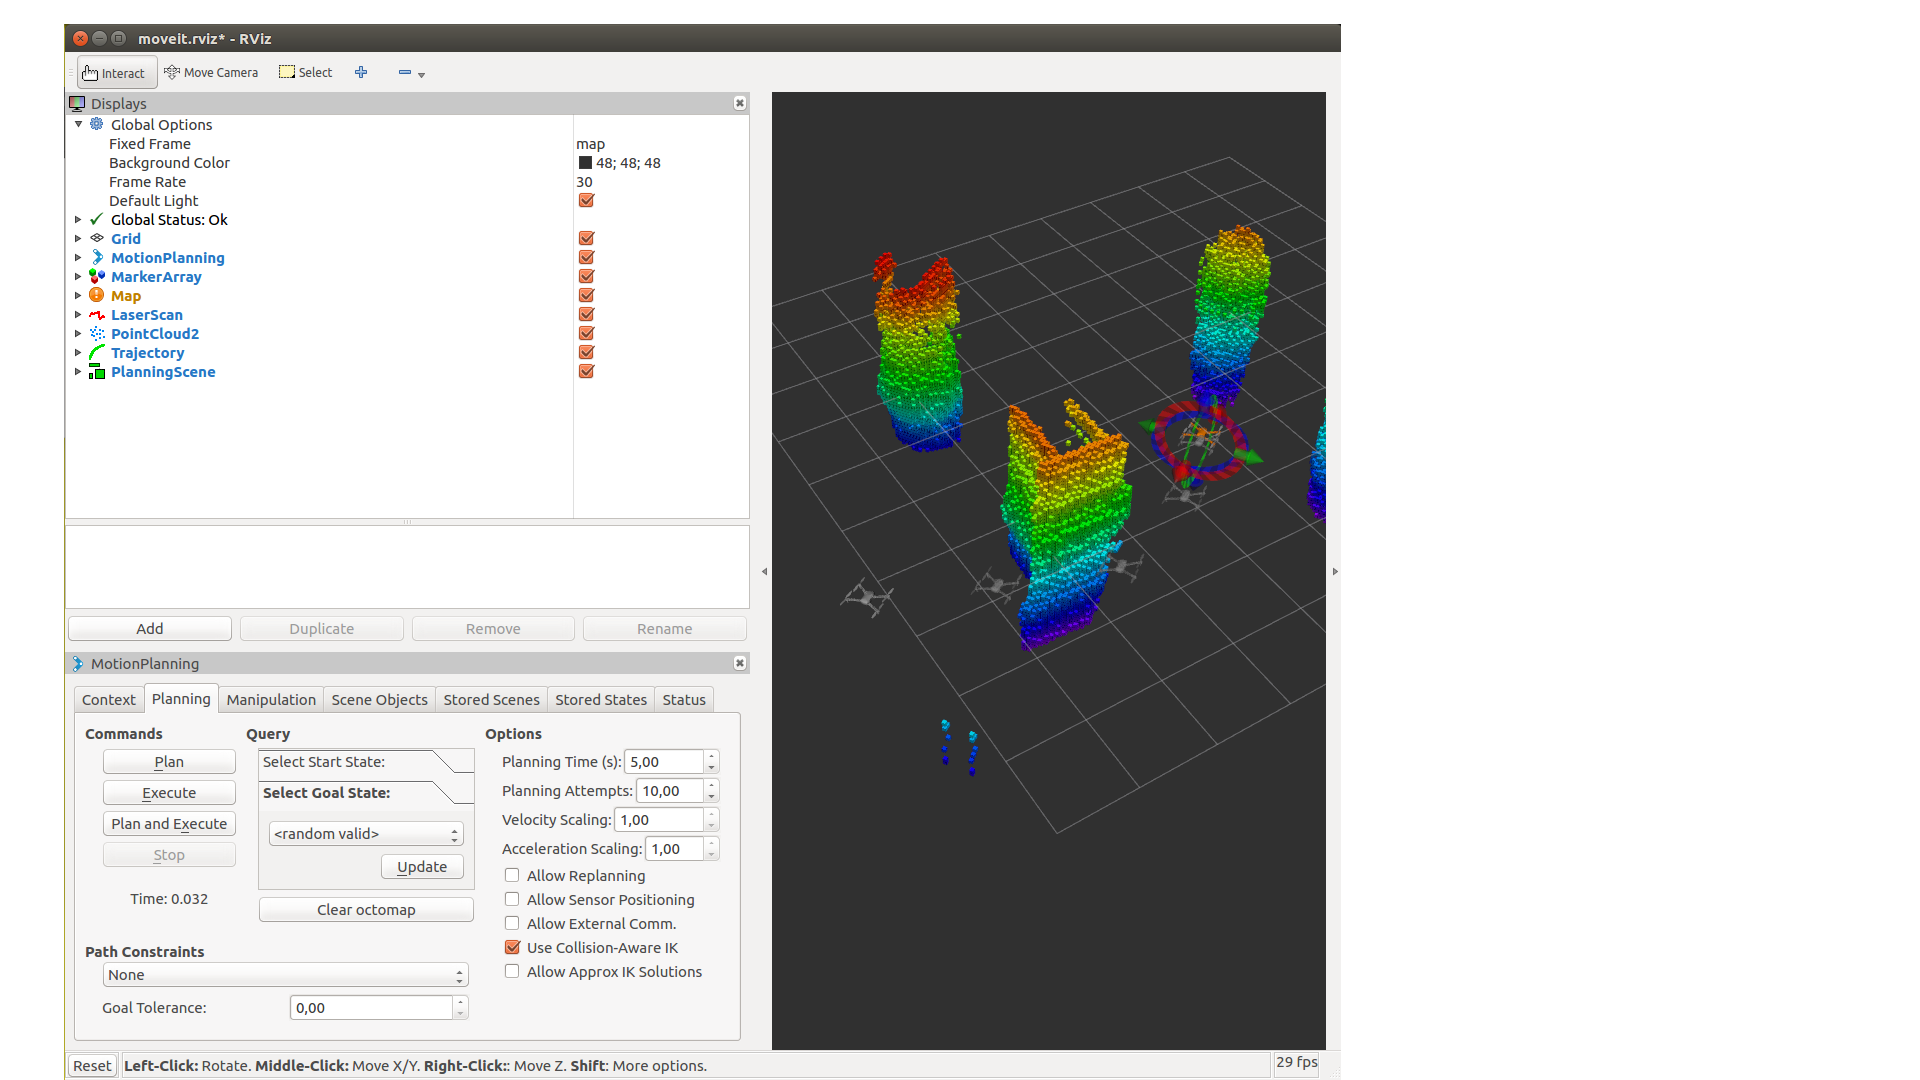
\includegraphics[width=0.9\linewidth]{img/rviz.png}
		\end{subfigure}
		\begin{subfigure}{0.4\textwidth}
		\centering
		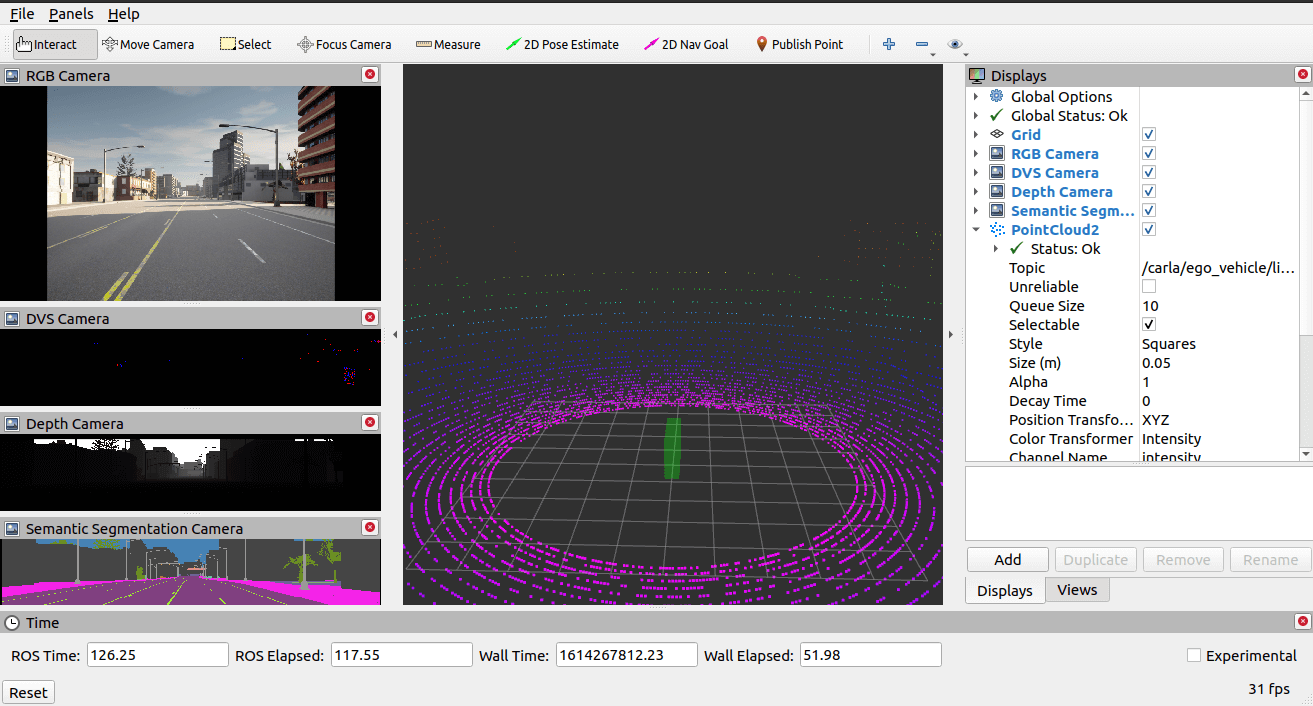
\includegraphics[width=0.9\linewidth]{img/rviz2.png}
		\end{subfigure}
		\captionof{figure}{Examples of visualization of ROS data with Rviz}
	\end{figure}
	\item \textbf{rosdep} is a dependency installer utility.
	\item \textbf{sros2} is a package that provide the tools and instruction to apply security on DDS.
\end{itemize}
Another tools that are connected with ROS and helps develop is the simulation environments. They allow to test the code on a simulated robot in different condition to find possible bugs in the code that if there was launched on a real robot can be harmful to it or the environment. They provide realistic physical mechanics at all the parts of simulation and in the documentation of ROS there are listened 2: Gazebo and Webots.
The first one is also a project under the Open Robotics and for a lot of projects is the default used like the one we will use.
Gazebo offer:
\begin{itemize}
	\item \textbf{ROS Integration} a bridge to converts the protobuf messages to ROS.
	\item \textbf{Performance tools} that allow to have it distributed on servers, dynamically asset loading and control of the time step for simulation to have the best performances.
	\item \textbf{Realistic simulation} that allow to insert a variety of sensor with their noise in a 3D rendering word built on Ogre 2.1\footnote{\href{https://wiki.ogre3d.org/Home}{https://wiki.ogre3d.org/Home}} and with the physic engine DART\footnote{\href{https://dartsim.github.io/}{https://dartsim.github.io/}}.
	\item \textbf{Extensibility} because its built on modularity, it allow with plugins to run code that interact with the simulation.	
\end{itemize}
	\begin{figure}[h]
		\centering
		\begin{subfigure}{0.4\textwidth}
			\centering
			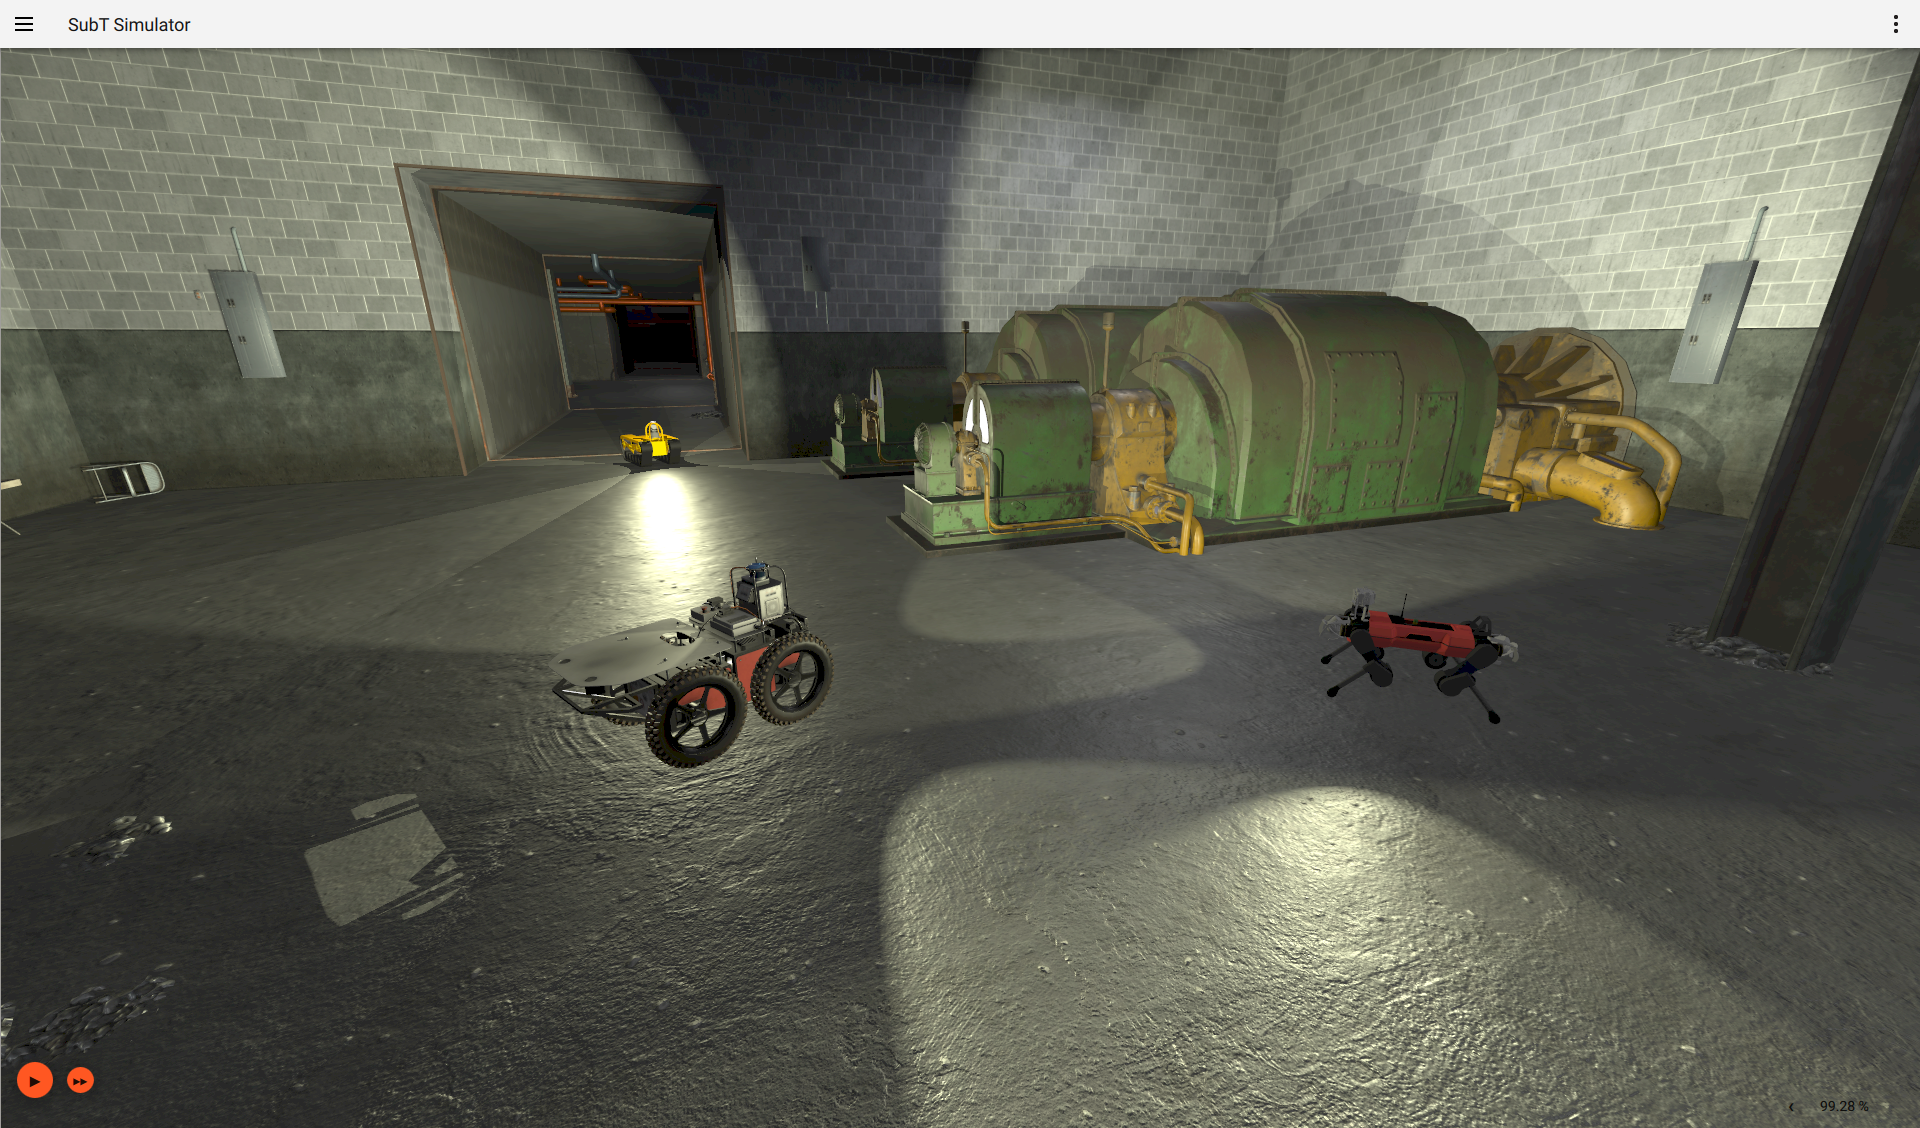
\includegraphics[width=0.9\linewidth]{img/gazebo1.png}
		\end{subfigure}
		\begin{subfigure}{0.4\textwidth}
			\centering
			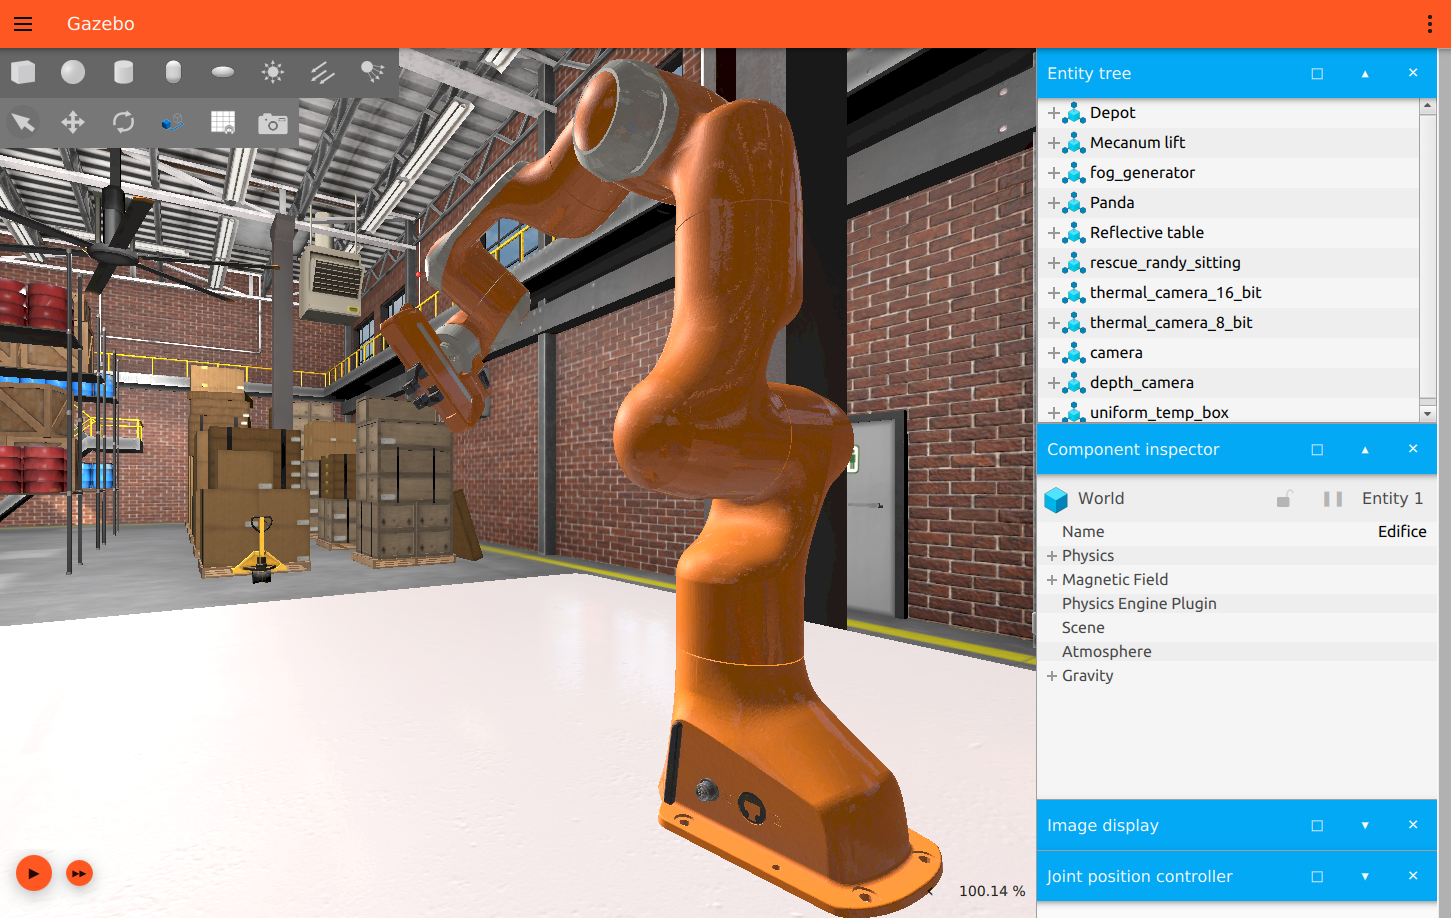
\includegraphics[width=0.9\linewidth]{img/gazebo2.png}
		\end{subfigure}
		\captionof{figure}{Examples of Gazebo}
\end{figure}
\chapter{Introduction to NAV2 and Google Cartographer}
Multiple tools are available for move a robot in an environment. The one that give a full system is Nav2
\footnote{\href{https://docs.nav2.org/}{https://docs.nav2.org/}}
\cite{macenski2020marathon2}
 the successor of ROS Navigation Stack of ROS 1.
\section{Description of Nav2}
Nav2 gives all the tools (perception, planning\cite{macenski2023survey}, control, localization, visualization) for whichever robot to navigate autonomously and reliably also thought hard environment. It allow to build a model of the environment from the data of the sensors, calculated dynamically the best path to follow to avoiding obstacles using a map, set the velocity of the motors and allow to follow logic step using a behaviors tree.
\begin{figure}[h]
\centering
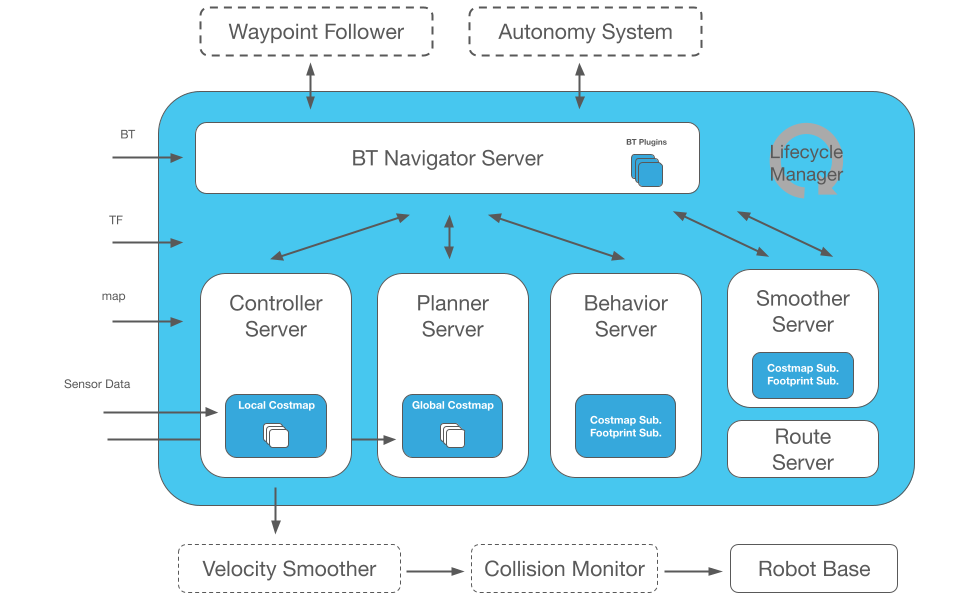
\includegraphics[width=0.8\linewidth]{img/nav2_architecture.png}
\captionof{figure}{Nav2 architecture}
\end{figure}
\newline
These are also some of the updates that have changed from ROS 1 other less notable changes are the use of:
\begin{itemize}
	\item \textbf{Behavior trees}\cite{Colledanchise_2018}: gives to Nav2 a structure for completing a series of tasks in a human readable way. Their structure is similar to a tree and allow to create complex system that can be tested with different tools. The package used for this is BehaviorTree.CPP\footnote{\href{https://www.behaviortree.dev/}{https://www.behaviortree.dev/}} that respect others allow to link different tree.
	\item \textbf{nav2\_util LifecycleNode} is a wrapper of rclcpp\_lifecycle LifecycleNode of the standard structure of ros as described in Nodes \ref{LifecycleNode} and add a bond connection to the lifecycle manager, node that knows the states of each node, and allow to  transition down its lifecycle nodes for safety if some node has crashed.
	\item \textbf{Action Server}: the functionality are described in the structure of ROS \ref{Action} and they are implemented in Nav2 for the interaction with the Behavior Tree (BT) like NavigationToPose (move to a location), NavigationThroughPoses (allow to select multiple waypoints), etc.
\end{itemize}
The control is based on this nodes:
\begin{itemize}
	\item \textbf{controller\_server} is the node that handle the request for moving the robot, using tree plugins progress checker (check if the robot has make some progress in following the path), goal checker (check if the robot has reached the goal position) and controller (generate the velocity command using the \textbf{local costmap} to move the robot avoiding collision)
	\item \textbf{planner\_server} is the node that handle the request for calculate the path, using a loaded plugin planner, to reach a position using the \textbf{global costmap} and the data from sensors.
	\item \textbf{bt\_navigator} is a Behavior Tree-based implementation of navigation that implement the NavigateToPose, NavigateThroughPoses, and other task interfaces to increment the flexibility during navigation.
	\begin{figure}[h]
		\centering
		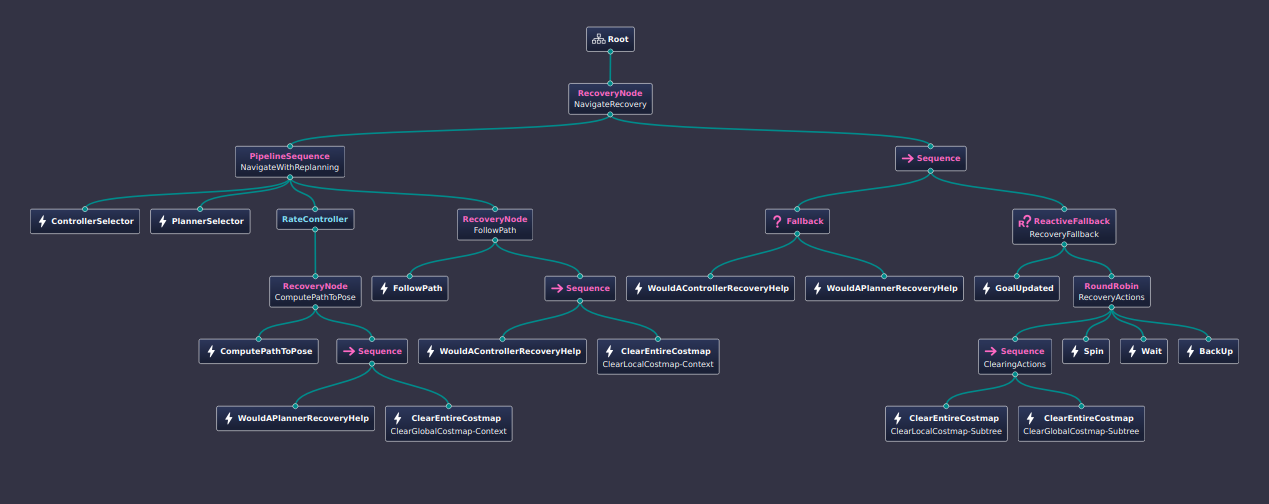
\includegraphics[width=0.8\linewidth]{img/bt2_nav2.png}
		\captionof{figure}{Nav2 bt navigation TOCECK}
	\end{figure}
	\item \textbf{smoother\_server}
	\item \textbf{behavior\_server}
	\item \textbf{waypoint\_follower}
	\item \textbf{velocity\_smoother}
	\item \textbf{global\_costmap}
	\item \textbf{local\_costmap}
\end{itemize}
\section{Cartographer}
\chapter{Review of related work on porting navigation stack from ROS1 to ROS2}
\chapter{Overview of open source fleet management systems, particularly Open-RMF}
\section{Open-RMF description}
...



